The goal of the thesis is to enable run-time state migration between applications serving the same purpose which are developed for different platforms and by different vendors. 
For this, a model-driven approach, as outlined in Figure \ref{fig:solution}, shall be developed. 
This approach shall allow adapting existing applications so that they support run-time state migration.
To do so, relevant types of possible run-time states for an application shall be modeled as in terms of an \textit{Application State Model} (see \fcircone).
An \textit{Application State Modeling Language} (see \fcirctwo) is needed to describe \textit{Application State Models}.
An \textit{Application State Model} can be common to multiple applications serving the same purpose. 
For instance, an \textit{Application State Model} for an e-mail application can be valid for multiple e-mail applications, e.g., K-9 Mail for Android and Mailspring for desktop operating systems. 
If two applications support the same state model, it shall be possible that a \textit{Run-time State} (see \fcircthree), which is an instance of an \textit{Application State Model}, can be extracted from the source application (see \fcircfour) and be injected into the target application (see \fcircfive). 
The approach focuses on interactive applications for end-users and shall be extensible in the sense that if a new application with serving the same purpose supports the same \textit{Application State Model}, migration from and to this application shall be supported as well. It is out of scope for the thesis to support run-time state migration between applications for which no common \textit{Application State Model} can be found. 

To enable run-time state migration, developers should develop an \textit{Application State Model} (or use an existing one) and add support for injecting and extracting run-time states to their applications. 
To simplify this, special libraries shall be developed that provide the basic functionality of run-time state migration, such as providing an API for validation, injection, and extraction.
The \textit{Application State Model} defines which types of \textit{Run-time States} can occur at run-time.
These libraries shall be able to validate the \textit{Run-time States} based on an \textit{Application State Model}.
When being integrated into an application, the supported \textit{Application State Models} need to be coupled to the applications by defining how the different types of \textit{Run-time States} are being injected and extracted.
To do so, an interface that is derived based on the \textit{Application State Model} needs to be implemented.
However, this coupling of the state model to a respective application is highly application-specific and needs to be implemented for each application by their developers or someone who has access to the source.
These libraries have to exist for the different programming languages in which source and target applications are written. 

If devices are in the same local network, these libraries establish a point-to-point connection. Otherwise, they use middleware to communicate over the internet.
For the indirect solution, a middleware shall be developed to which applications can introduce themselves to communicate with other same-purpose applications supporting the same \textit{Application State Model}. 
The library uses the developed interface at run-time to extract the \textit{Run-time State} of the source application. The library shall pass \textit{Run-time State} to a target application, either directly or with the help of middleware. 
Developers are responsible for enhancing target application so that the library can validate and inject \textit{Run-time State} to it. 
For this, they have to change the state of target application based on the received \textit{Run-time State} (e.g., adjusting or placing data in a proper position on the UI). 

To show the feasibility of the approach, as part of the thesis, two open-source e-mail clients shall be adapted to support run-time state migration based on the developed approach. These applications shall be for different platforms, and their source code should be freely accessible to allow the integration of the library.
Suggestions for e-mail clients to be adapted are K-9 Mail for Android and Mailspring for desktop operating systems.
K9-Mail Android application is developed in Java; therefore, it requires an Android library. Moreover, Mailspring is developed using Node.js for desktop operating systems, and it needs a JavaScript library.

\FloatBarrier
\begin{figure}[!b]
    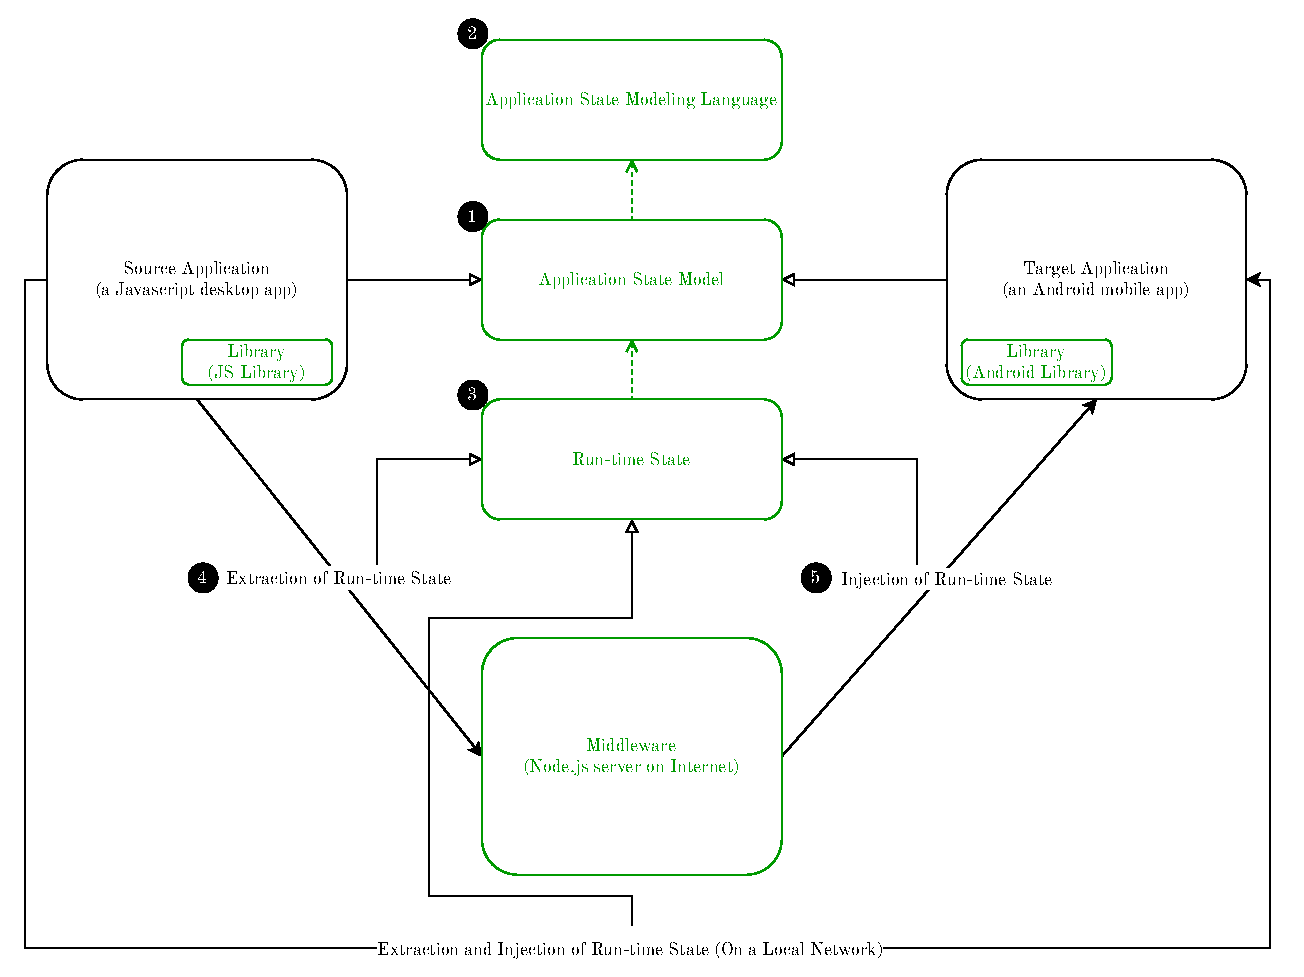
\includepdf[width=\linewidth, offset= 0 -100]{figures/solution.pdf}
    % \vspace{10cm}
    \caption{Showing the approach of run-time state migration between two applications.}
    \label{fig:solution}
\end{figure}
\FloatBarrier
